\subsection{JudasNET}

\texttt{JudasNET} is the architecture of choice for interpreting data

\begin{figure}{h}
    \centering
    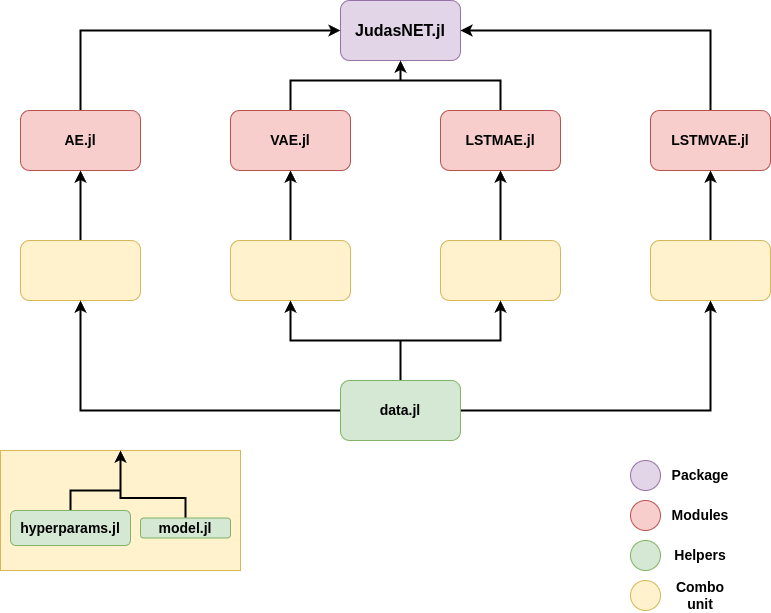
\includegraphics[scale=.6]{figures/judasnet.png}
    \caption{Flowchart over JudasNET}
    \label{fig:judasnet}
\end{figure}

\subsubsection{Modification to Flux.jl}

As mentioned previously, one of the main benefits with Julia packages is the ability to easily add new functionality to packages. When working with \texttt{Flux.jl}, this has certainly been useful. For our research, we had to write our own LSTM functors to be able to achieve a LSTM Autoencoder.  \\

The first of this functors is a regular LSTM, but with \texttt{relu} as the activation function for the different gates. Secondly, we rewrote the TimeDistributed layer \cite{keras} for Flux since there is no corresponding alternative as of the writeday of this paper. The final layer we had to recreate is what's known as a \texttt{RepeatVector} in Keras. When we have all of these together, we can finally put them together and write our model. 

\begin{figure}[h]
    \centering
    \lstinputlisting[language=Julia]{code/judasnet.jl}
    \caption{JudasNET flux model}
    \label{fig:fluxjudasnet}
\end{figure}